\documentclass[es,practica]{uah}

\usepackage{subfigure}

\tema{V1}
\titulo{Introducción a la imagen digital}{}

\begin{document}

\titulacion{Grados Informática}
\asignatura{Sistemas Audiovisuales y Aplicaciones Multimedia}{}
\curso{2021/2022} 

\maketitle

\section{Introducción}

\subsection{Imagen digital}

Una imagen es una representación bidimensional de la cantidad de luz recibida por un sistema de percepción visual, por ejemplo una cámara de vídeo o el ojo humano, en función de la dirección de incidencia. Una imagen digital se corresponde con la digitalización de la señal anterior. En el proceso de digitalización se establecen los parámetros más importantes de una imagen digital:
\begin{enumerate}
	\item {\bf Dimensiones y resolución de la imagen}: Al digitalizar una imagen, debemos muestrear ésta en ambas dimensiones (horizontal y vertical). Cada una de las muestras recibe el nombre de píxel, y las dimensiones de la imagen indican el número de píxeles que componen la imagen, en horizontal y vertical. Cuanto mayor sea el número de píxeles, mayor será la ``calidad'' de la imagen, pero mayor será también el tamaño del archivo que la almacena. Cuando hablamos de la impresión de una imagen, por ejemplo, en papel fotográfico o en un documento, la resolución se refiere al número de píxeles por unidad de superficie del papel, siendo la unidad más empleada los dpi (dots per inch), o ppp (píxeles por pulgada). Así pues, la resolución relaciona la dimensión de la imagen con el tamaño de impresión de ésta. Los valores más comunes suelen ser:
	\begin{itemize}
		\item Impresión en papel fotográfico: 300 a 400 dpi.
		\item Impresión en papel: 150 dpi.
		\item Impresión en póster: 50 dpi.
	\end{itemize}

	Si la resolución de la imagen baja por debajo de los valores indicados arriba, la calidad de la imagen se reduce considerablemente, produciéndose el efecto denominado pixelado, como se muestra en las figuras \ref{fig:fig7} y \ref{fig:fig8}.

\begin{figure}[h!]
	\centering
	\begin{subfigure}
	  \centering
	  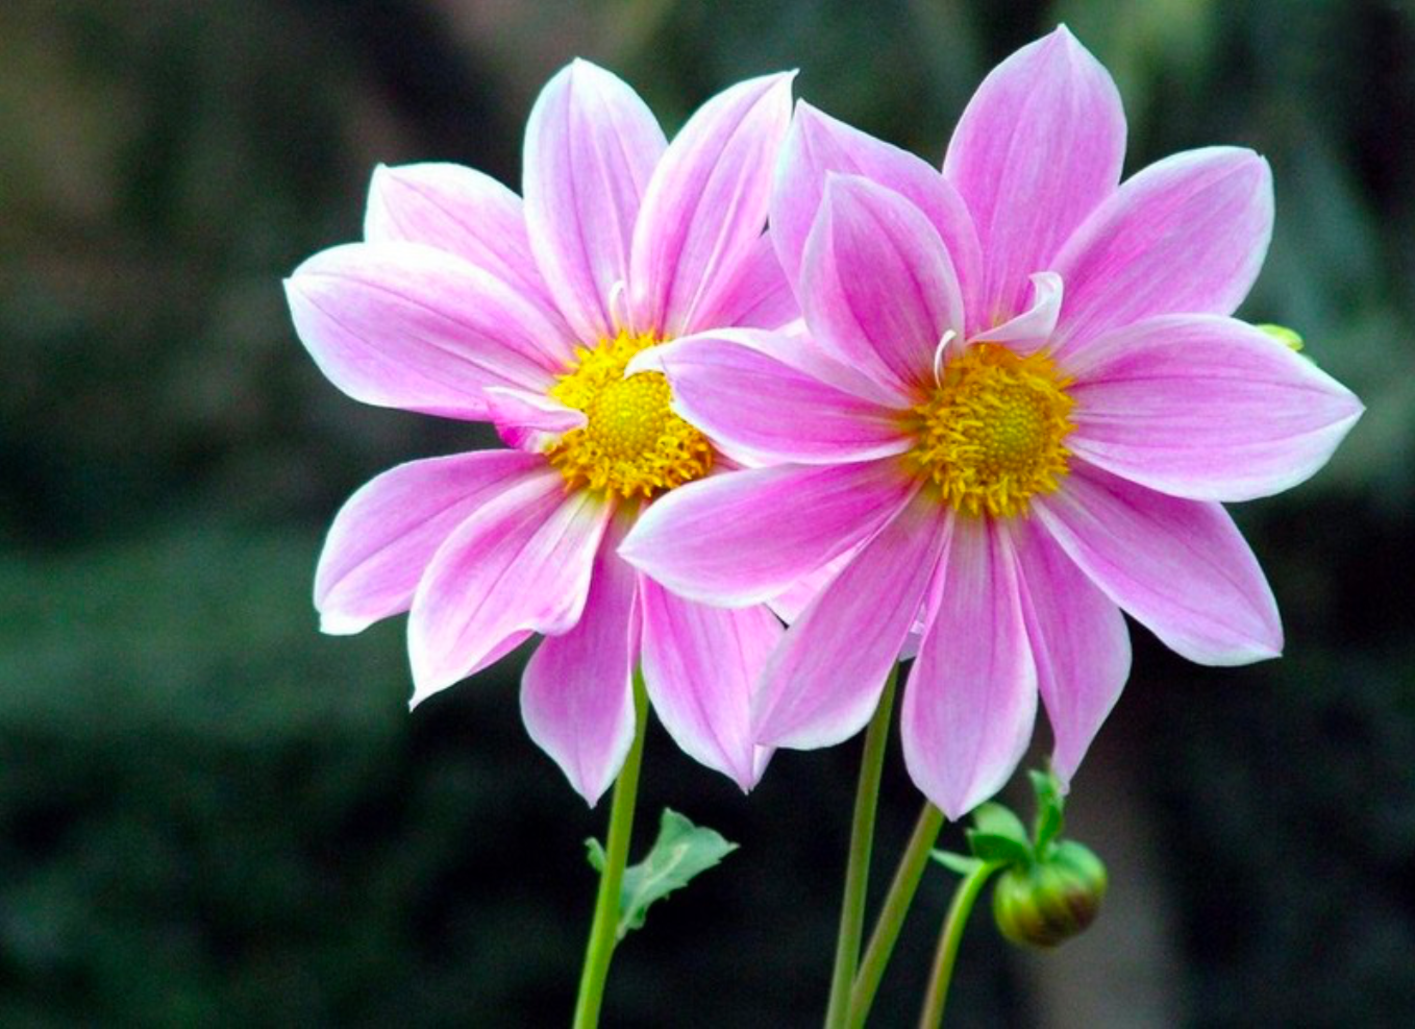
\includegraphics[width=4cm]{Figuras/Figura7}
	  \caption{Imagen con resolución aceptable}
	  \label{fig:fig7}
	\end{subfigure}
	\begin{subfigure}
	  \centering
	  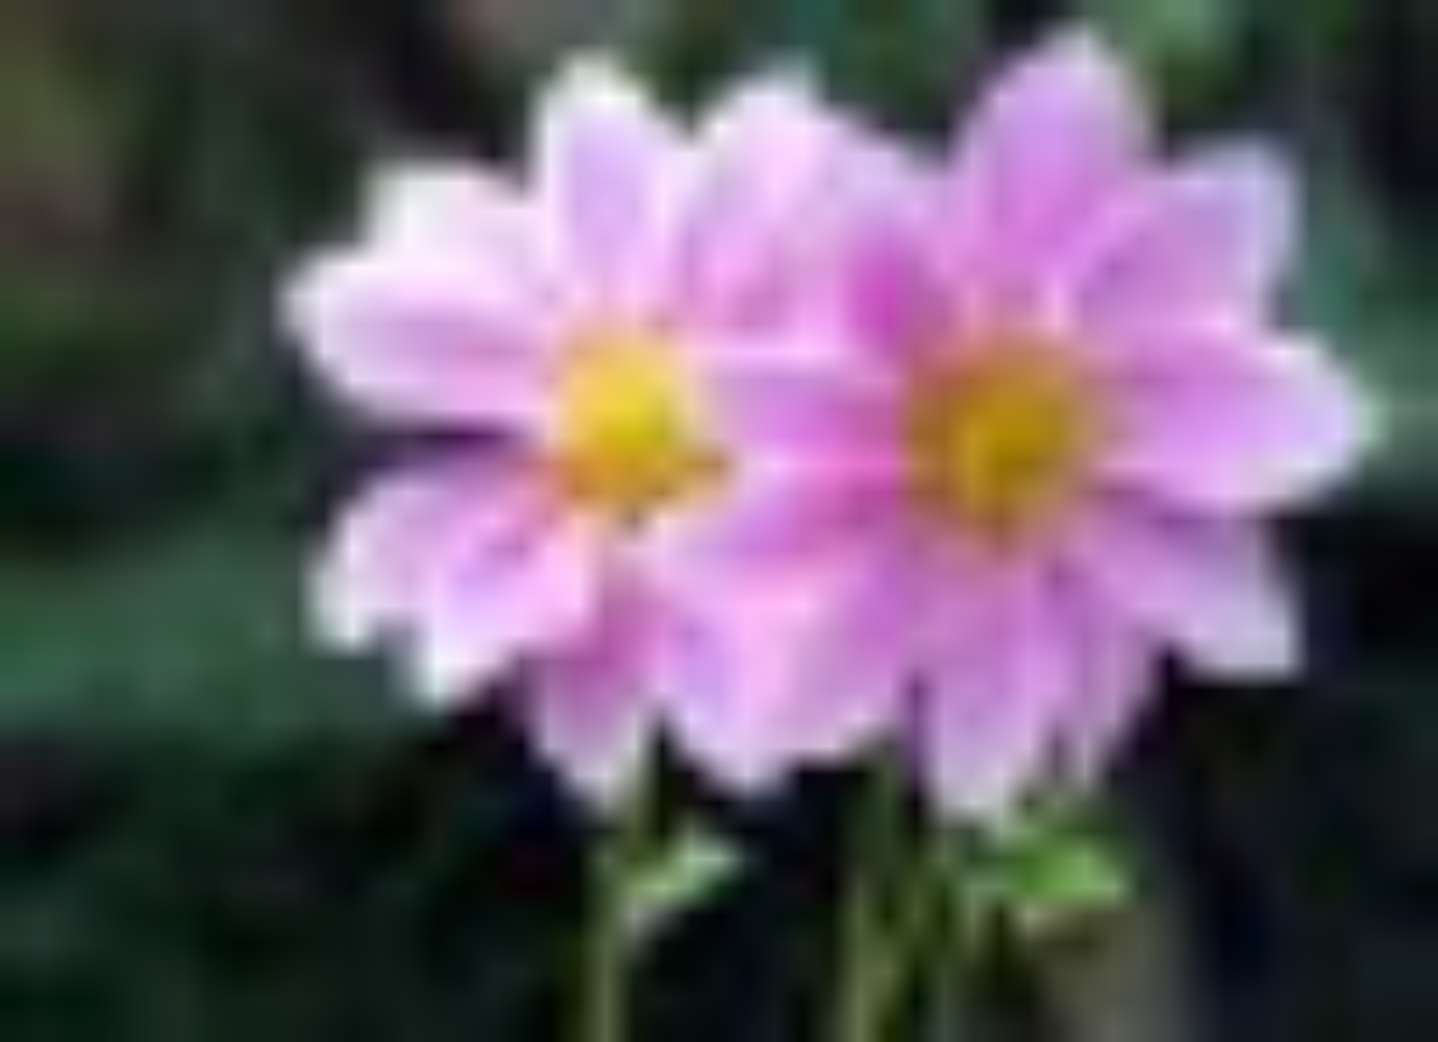
\includegraphics[width=4cm]{Figuras/Figura8}
	  \caption{Imagen con efecto de pixelado}
	  \label{fig:fig8}
	\end{subfigure}
	\caption{Ejemplo de distintas resoluciones de imagen}
	\end{figure}
	
	Cuando la imagen va a ser representada en un sistema digital, como la pantalla de un ordenador o un televisor, la resolución carece de sentido, ya que cada píxel de la imagen se corresponde con un píxel de la pantalla.
	
	\item {\bf Profundidad de píxel}: Al digitalizar cualquier señal, se necesita cuantificar la señal, lo que implica determinar cuántos bits se utilizarán para representar cada muestra. En el caso de las imágenes, este valor suele denominarse como profundidad de píxel, siendo el valor más común el de 8 bits (1 byte) por píxel, aunque otros valores también pueden ser empleados. Valores por encima de 8 bits requieren mayor capacidad para el almacenamiento de la imagen sin un aumento apreciable de la calidad de la imagen. Valores por debajo de 8 bits pueden provocar la aparición de bandas de color, como se muestra en las figuras \ref{fig:fig9} y \ref{fig:fig10}.

\begin{figure}[h!]
	\centering
	\begin{subfigure}
	  \centering
	  
\includegraphics[width=4cm]{Figuras/Figura9}
	  \caption{Degradado con 8 bits por pixel}
	  \label{fig:fig9}
	\end{subfigure}
	\begin{subfigure}
	  \centering
	  
\includegraphics[width=4cm]{Figuras/Figura10}
	  \caption{Degradado con 4 bits por pixel}
	  \label{fig:fig10}
	\end{subfigure}
	\caption{Ejemplo de distintas profundidades de bits por pixel}
	\end{figure}

\end{enumerate}

\subsection{Imágenes en color. Espacios de color}

La sensación de color es percibida por el cerebro gracias a que la retina del ojo humano está compuesto por células sensibles a colores (longitudes de onda) distintos. Así, existen células sensibles al color rojo, células sensibles al color verde y células sensibles al color azul. Mediante la composición de la información recibida por cada una de las células anteriores, el cerebro es capaz de interpretar el color correspondiente. Así pues, para poder formar una imagen en color, necesitamos almacenar por cada píxel la información del color rojo, del color verde y del color azul.


\begin{figure}[h!]
  \centering
  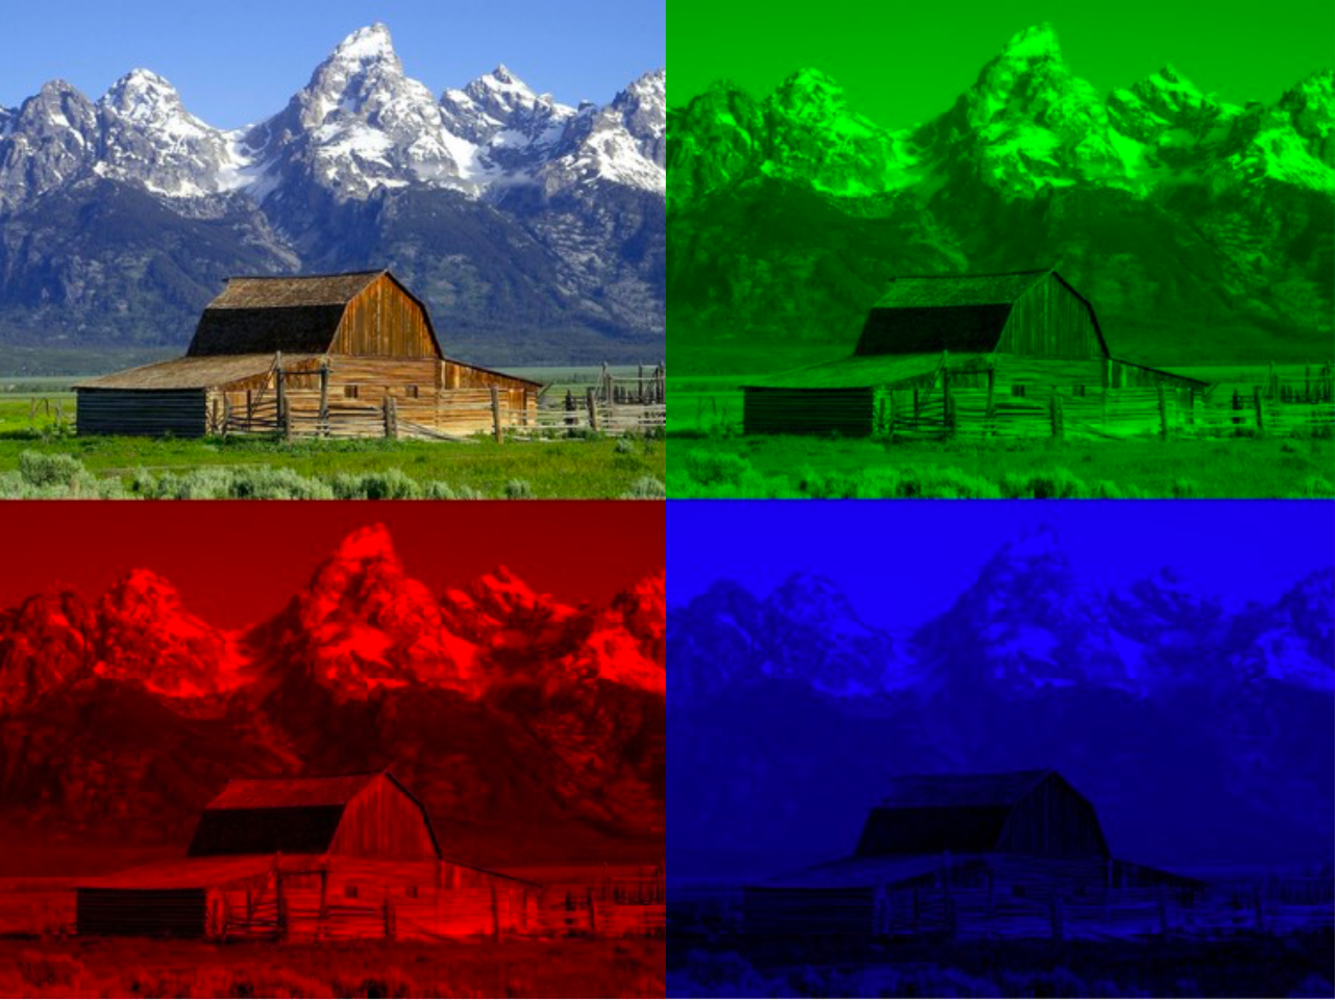
\includegraphics[width=5cm]{Figuras/Figura11}
  \label{fig:fig11}
\end{figure}


Si tenemos en cuenta que lo más común es emplear 8 bits para almacenar cada una de las componentes de color, podemos determinar que cada píxel necesitará 24 bits para ser almacenado, en lugar de los 8 bits que necesitan las imágenes en escala de grises.

Aunque el formato más simple para representar una imagen en color es, como se ha indicado anteriormente, cada uno de los canales de color de forma independiente, ésta no es la única forma de hacerlo. Así pues, a partir de la información de rojo, verde y azul podemos obtener la cantidad total de luz (luminancia) y el color (crominancia) de cada píxel. De esta forma, en función de cómo se represente el color, hablamos del espacio de color.

Si representamos cada uno de los colores por separado, hablamos de espacios de color basados en colores primarios. Dentro de este bloque, tenemos el RGB (red, green, blue) empleado para los monitores, el CMY (modelo complementario al RGB) y el CMYK (cian, magente, yellow, black) extensión del CMY, comúnmente empleado para impresión en papel.

Una forma de visualizar toda la paleta de colores del espacio RGB es el llamado cubo RGB, como el de la figura. Si consideramos un sistema de coordenadas cartesianas de 3 dimensiones, uno de los ejes sería el rojo (R), otro el azul (B) y otro el verde (G). Mediante la combinación lineal de las 3 componentes podemos representar todos los colores posibles. En este cubo, el origen de coordenadas sería el negro (parte posterior del cubo, no visualizado en la figura anterior), el vértice opuesto el blanco, y la línea que une ambos extremos sería la escala de grises.

\begin{figure}[h!]
  \centering
  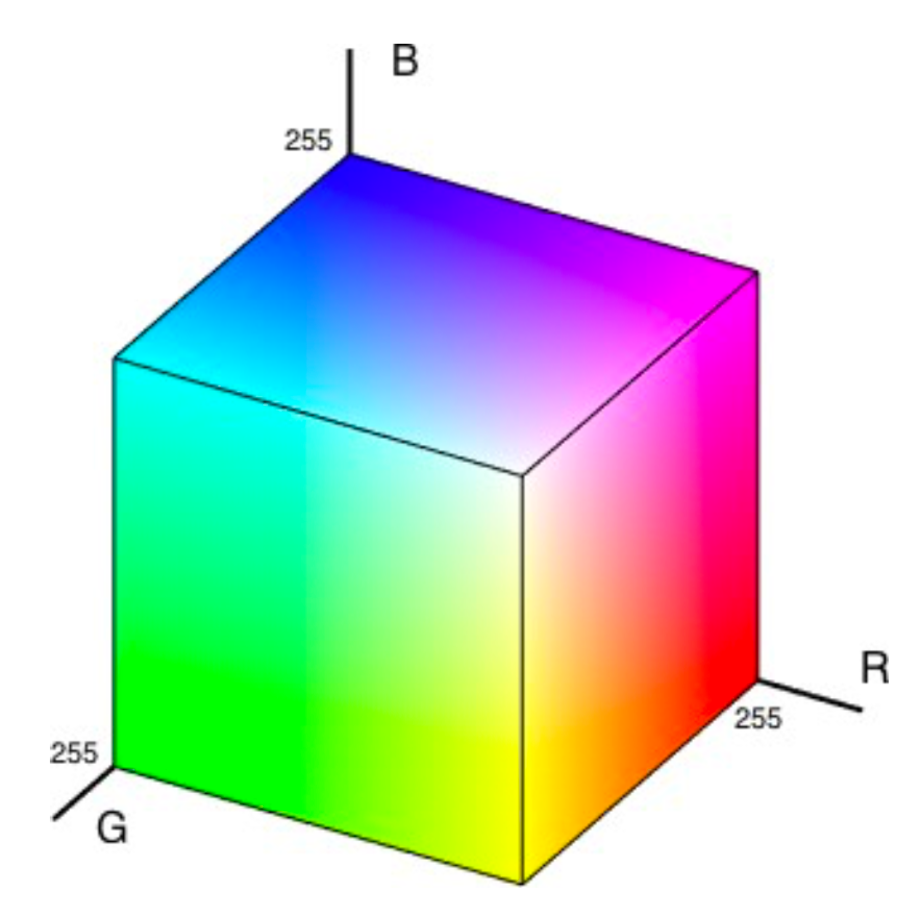
\includegraphics[width=5cm]{Figuras/Figura12}
  \caption{Cubo RGB}
  \label{fig:fig12}
\end{figure}


Finalmente, tenemos los modelos de color basados en la percepción del color por el hombre. En este caso, el color se descompone en valor (intensidad o cantidad de luz), tono o matiz (color) y saturación (mezcla del color con el blanco). Entre estos espacios de color, podemos enumerar el HSI o el HSV. Por ejemplo, en la representación visual del cono HSV de la figura, la altura con respecto al extremo inferior del cono es el valor, la distancia en sentido horizontal con respecto al eje del cono es la saturación, y el ángulo con respecto a un eje de referencia es el matiz o color. En el espacio HSV, el ángulo se toma desde el color rojo, de tal forma que un ángulo de 0 grados (o 360 grados) corresponde al rojo, un ángulo de 120 grados al verde y de 240 grados al azul.

\begin{figure}[h!]
  \centering
  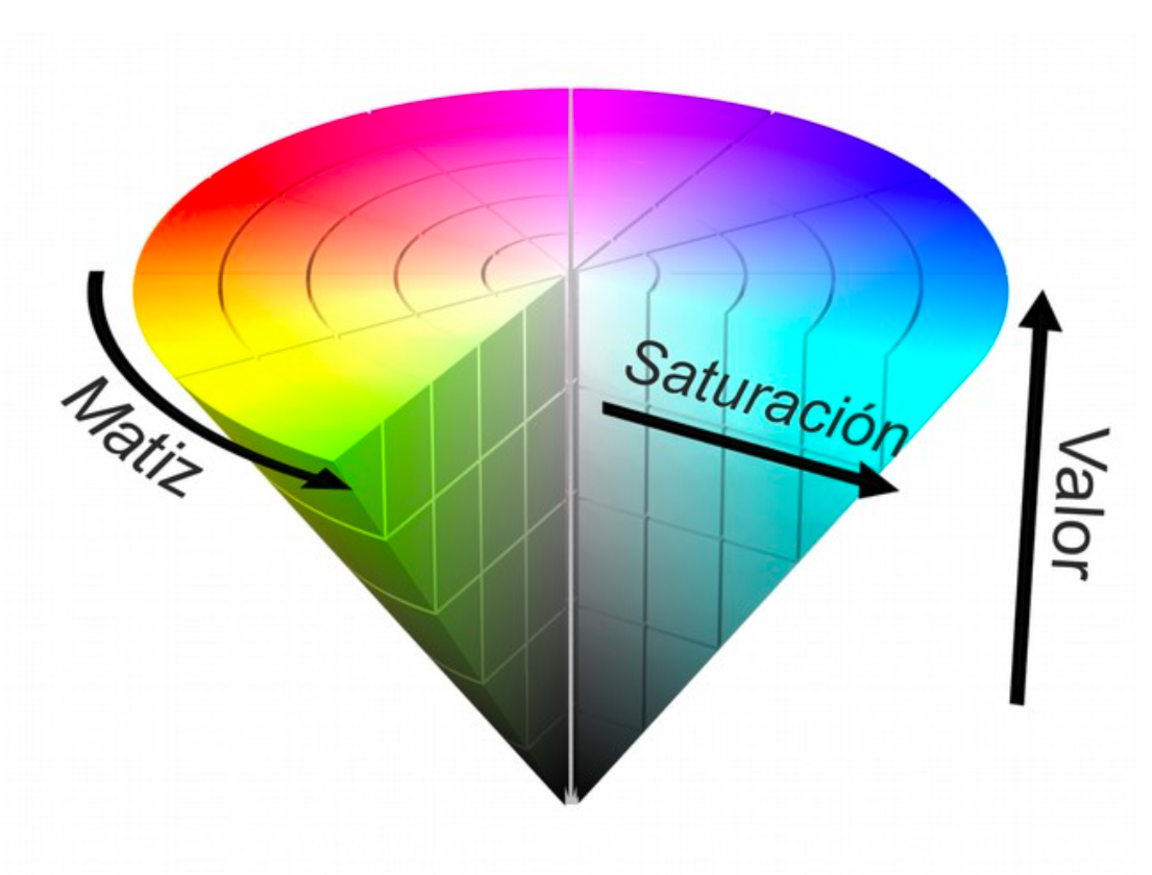
\includegraphics[width=5cm]{Figuras/Figura13}
  \caption{Cono HSV}
  \label{fig:fig13}
\end{figure}

\subsection{Vídeo digital}

La forma más simple de definir una señal de vídeo (sólo vídeo, sin audio) es como una secuencia de imágenes (fotogramas) consecutivas. Por lo tanto, en la definición de un archivo de vídeo, aparte de los parámetros empleados a la hora de definir una imagen (dimensiones, profundidad de píxel, espacio de color), es necesario definir también la tasa de fotogramas (framerate), es decir, el número de fotogramas por segundo. En este sentido, es necesario que la tasa de fotogramas sea superior a un determinado valor, para poder crear la sensación de movimiento en el cerebro. En general, este valor debe estar por encima de 10 fps (frames per second). Algunos valores típicos son:
\begin{itemize}
	\item Cine: 24 fps
	\item Televisión analógica, sistema PAL: 25 fps
	\item Televisión analógica, sistema NTSC: 30 fps
	\item Televisión digital terrestre: 25 fps
	\item Slow Motion: > 200 fps (en grabación).
\end{itemize}

Con respecto a los parámetros relacionados con la imagen, mientras en fotografía estos no siguen un estándar claro, sino que dependen sobre todo del fabricante, en vídeo está bastante mejor definido, en concreto:
\begin{enumerate}
	\item Resolución: Se refiere al tamaño de los fotogramas, en píxeles. En vídeo digital, alguno de los estándares más populares son:
	\begin{itemize}
		\item VGA: 640 x 480
		\item HD: 1280 x 720
		\item Full HD: 1920 x 1080
		\item 4K: 3840 x 2160
	\end{itemize}
	\item Relación de aspecto: Se refiere a la relación entre el ancho y el alto de la imagen. Algunos estándares:
	\begin{itemize}
		\item VGA: 3:4
		\item TDT (HD, Full HD, 4K, ...): 16:9
		\item Cine: 2,39:1 y 1,85:1
	\end{itemize}
	\item Espacio de color: Básicamente se emplea el YCbCr, que es la versión digital del estándar PAL analógico.
\end{enumerate}

\subsection{Contenedores multimedia}

Cuando hablamos de un archivo multimedia, debemos tener en cuenta que estamos tratando con distintos tipos de información en un mismo archivo. Así, un archivo multimedia suele contener vídeo y audio, pero también otro tipo de información, como subtítulos, capítulos, etc. De forma resumida, un contenedor multimedia se refiere a la forma en que se organiza (multiplexa) toda la información dentro de un archivo. De esta forma, debemos ser capaces de diferenciar entre el formato de vídeo, el formato de audio, el formato de subtítulos, etc y el formato del contenedor. Dentro del formato del contenedor, los más conocidos son:
\begin{itemize}
	\item AVI: Formato más común para archivos multimedia.
	\item MPEG-2 PS: Formato para DVD.
	\item MPEG-2 TS: Formato para transmisión mediante TDT.
	\item FLV: Transmisión de vídeo por internet (streaming). Empleado por ejemplo por YouTube.
	\item ASF: Formato para streaming, principalmente radio.
	\item MOV: Formato para edición de vídeo, propiedad de Apple.
	\item OGG: Formato abierto.
\end{itemize}


\section{Formatos}

El formato de una señal audiovisual se refiere a la forma en que la información (audio, vídeo, imagen) es almacenada y/o transmitida. Para cada una de los tipos de contenidos, existen distintos formatos, y el parámetro más importante está relacionado con si la información es comprimida o no para reducir su tamaño. Así pues, existen tres tipos de formatos, en función del tipo de compresión realizada
\begin{itemize}
	\item Sin compresión: la información se almacena tal cual, sin realizar ningún tipo de manipulación orientado a reducir su tamaño. La principal ventaja es que al no requerir de ningún tipo de procesado, su codificación y decodificación es más rápida. Por contra, el tamaño del archivo resultante no queda reducido y su tamaño puede ser elevado.
	\item Compresión con pérdidas: se tratan de procedimientos en los que la señal resultante no es exactamente igual a la señal original. No obstante, si las diferencias no son muy grandes, dicha diferencia no será apreciable. La principal ventaja es que consigue una reducción del tamaño del archivo muy elevada. El principal inconveniente es que si la diferencia con respecto a la imagen original es grande, se producirá una distorsión en la señal que podrá ser apreciable.
	\item Compresión sin pérdidas: en este caso, se emplean algoritmos de compresión que consiguen reducir el tamaño del archivo, sin causar pérdidas en la información, esto es, la señal resultante es exactamente igual a la señal original. El principal inconveniente es que la reducción en el tamaño del archivo es generalmente menor que con los formatos de compresión con pérdidas.
\end{itemize}

Relacionado con la compresión de señales audiovisuales, aparecen los conceptos de tasa de compresión y calidad de la señal.

\subsection{Tasa de compresión}

La tasa de compresión relaciona el tamaño del archivo una vez comprimido con el tamaño del archivo original, cuando éste no está comprimido. Por ejemplo, supongamos una imagen de 640 por 480 píxeles, con 8 bits por píxel, en color. En este caso, el tamaño del archivo original, sin compresión, sería:
\begin{displaymath}
	S=W\cdot H\cdot C\cdot P=640\cdot 480\cdot 3\cdot 8=7,03 Mbits=900 KBytes
\end{displaymath}

Si dicha imagen la guardamos en un formato con compresión, y el archivo correspondiente tiene un
tamaño de, por ejemplo, 120 KBytes, la tasa de compresión sería:

\begin{displaymath}
	T = 1 - \frac{120}{900} = 0.87 = 87\%
\end{displaymath}

Cuanto mayor sea la tasa de compresión, mayor será la reducción del tamaño del archivo. Evidentemente, los formatos sin compresión tendrán una tasa de 0\%.
Para las señales audiovisuales que varían en el tiempo, esto es, las señales de audio y vídeo, suele ser más frecuente el uso de la tasa de bit (bitrate) en lugar de la tasa de compresión, que es el parámetro más frecuentemente empleado con las imágenes. Recordemos que la tasa de bits, por ejemplo, de una señal de audio muestreada a 48 kHz, dos canales estéreo y 16 bits por muestra es de:
\begin{displaymath}
	b= 2 \cdot 48000 \cdot 16 \approx 1536 kbps
\end{displaymath}


Así, si la tasa de bits se redujese a, por ejemplo, 16 kpbs, la tasa de compresión sería:

\begin{displaymath}
	T = 1 - \frac{16}{1536} = 0.98 = 98 \%
\end{displaymath}

\subsection{Calidad de la señal}

Cuando hablamos de formatos de compresión con pérdidas, la señal obtenida después del proceso de compresión / descompresión es distinta a la original. Para cuantificar la diferencia entre ambas señales, se pueden establecer distintos parámetros de calidad. De entre todos, el más simple consistiría en calcular la relación señal a ruido a partir de la diferencia muestra a muestra entre ambas señales, y posteriormente el valor medio de dicha diferencia:
\begin{displaymath}
	SN = \frac{1}{M} \sum_i |A_i-B_i|
\end{displaymath}

donde A es la señal original, B la señal comprimida, y el sumatorio se realiza para todas las M muestras de la señal. En general, el valor suele expresarse en decibelios, para ello necesitamos calcular el logaritmo del valor anterior:
\begin{displaymath}
	SN = 20\cdot log \left ( \frac{1}{M} \sum_i |A_i-B_i| \right )
\end{displaymath}
En lugar del valor absoluto, en ocasiones también suele emplearse el cuadrado de la diferencia:
\begin{displaymath}
		SN = 10\cdot log \left ( \frac{1}{M} \sum_i (A_i-B_i)^2 \right )
\end{displaymath}




En general, suele establecerse el límite en unos 20 dB, de tal forma que para valores de SN por encima de ese valor la calidad de la señal se considera aceptable. Para valores por debajo, la calidad se reduce considerablemente, y comienzan a aparecer lo que se denomina como artefactos de compresión, tal y como se puede observar en las figuras \ref{fig:fig14} a \ref{fig:fig16}, para el caso de una imagen en color al comprimirla con el formato jpeg.


\begin{figure}[h!]
	\centering
	\begin{subfigure}
	  \centering
	  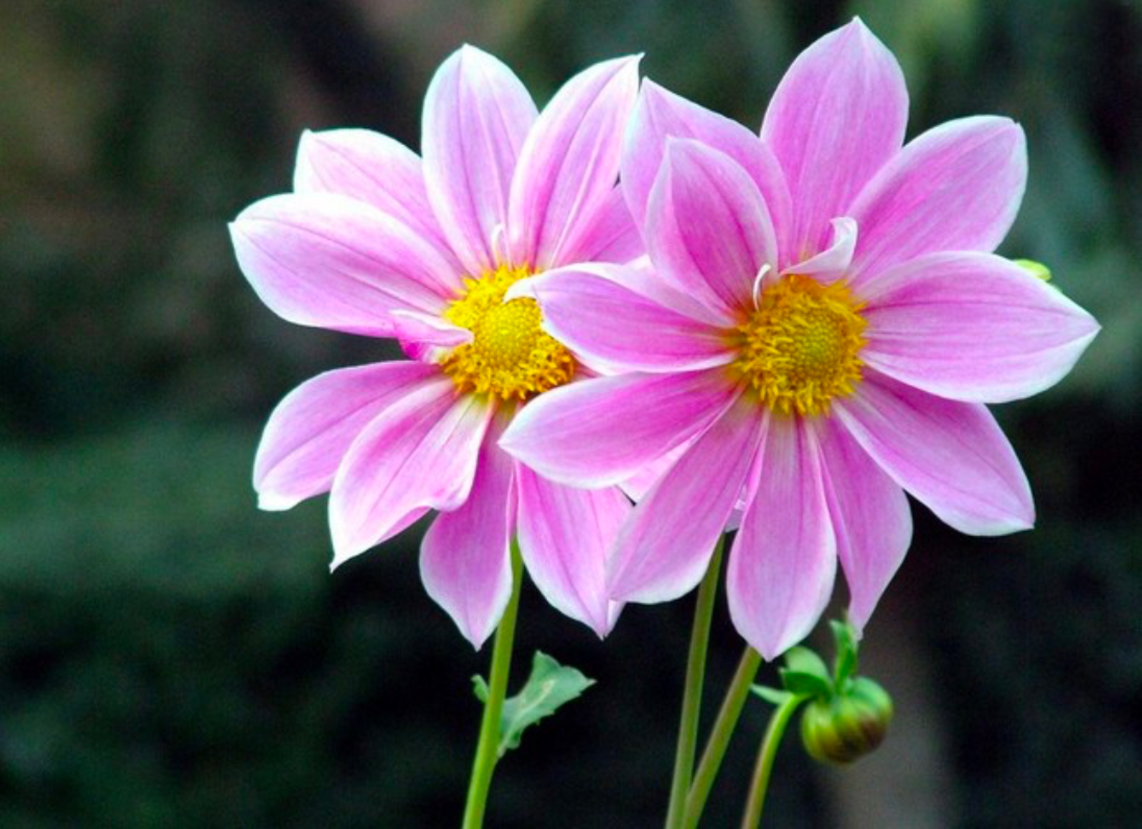
\includegraphics[width=3cm]{Figuras/Figura14}
	  \caption{Imagen original. Tamaño: 573 kBytes}
	  \label{fig:fig14}
	\end{subfigure}
	\begin{subfigure}
	  \centering
	  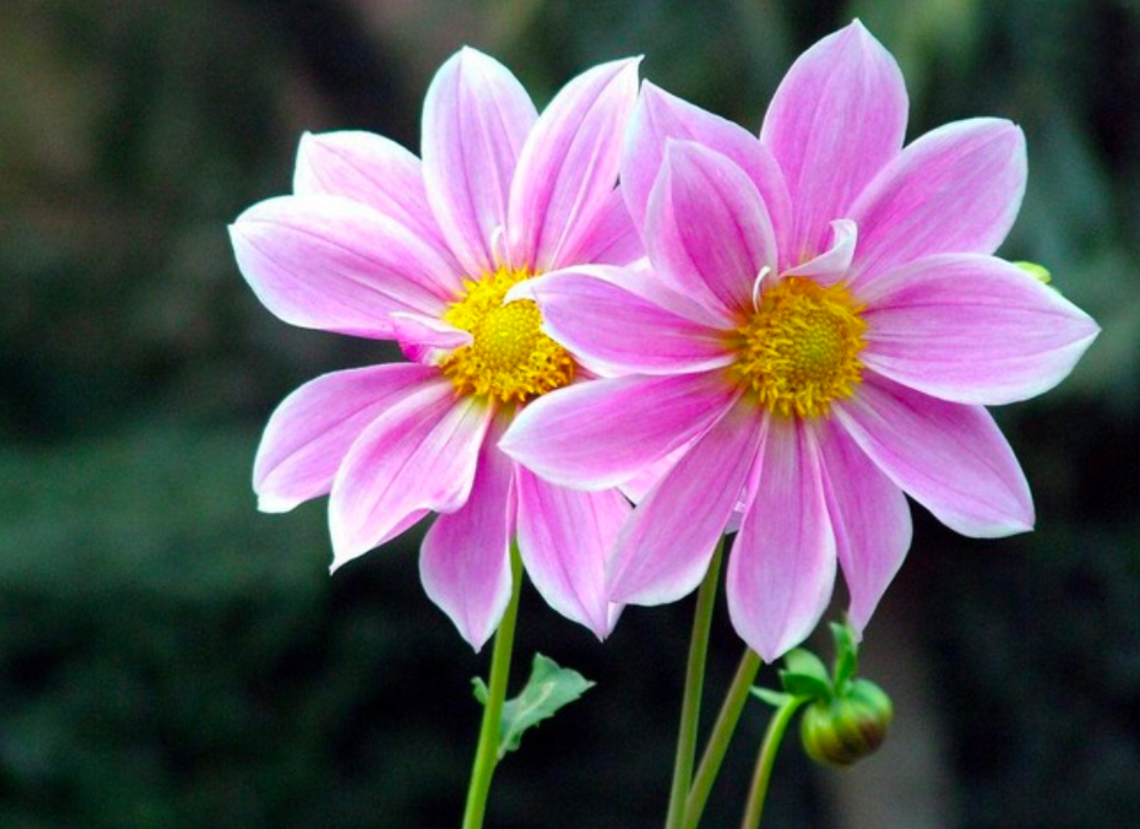
\includegraphics[width=3cm]{Figuras/Figura15}
	  \caption{Imagen comprimida jpeg. Tasa: 89\%}
	  \label{fig:fig15}
	\end{subfigure}
	\begin{subfigure}
		\centering
		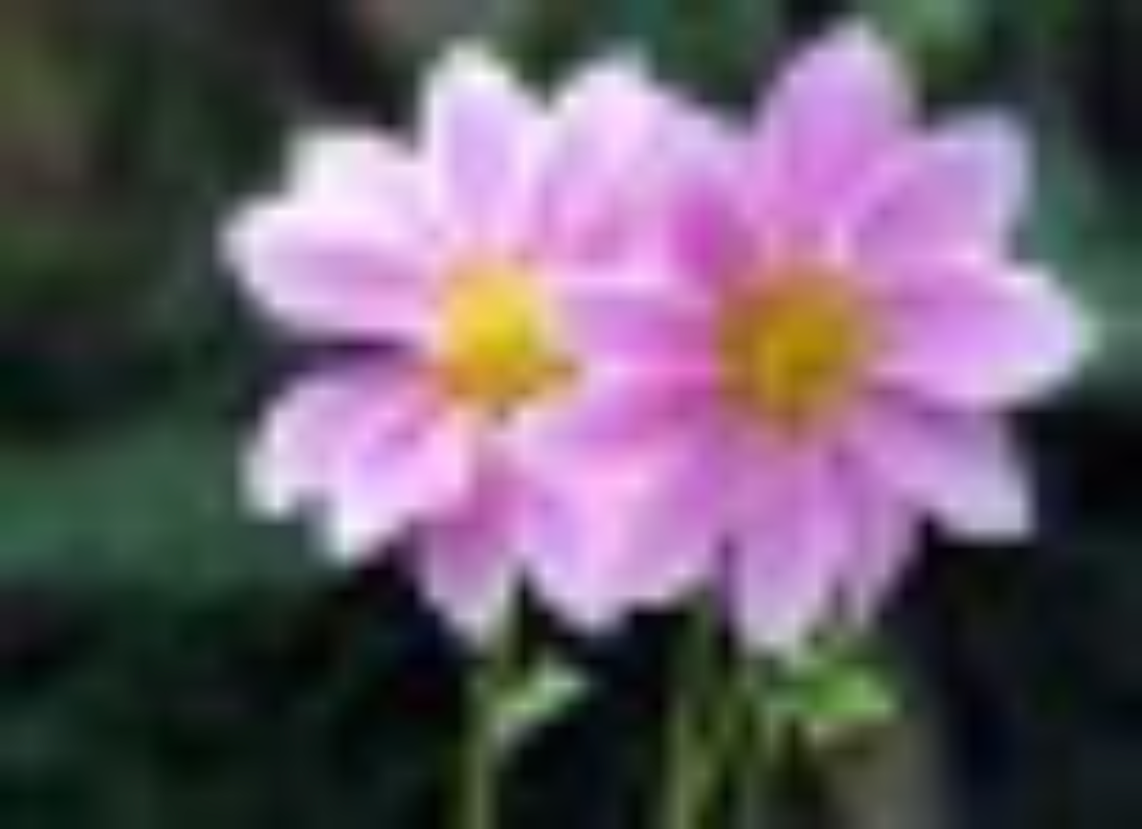
\includegraphics[width=3cm]{Figuras/Figura16}
		\caption{Imagen comprimida jpeg. Tasa: 98\%}
		\label{fig:fig16}
	  \end{subfigure}
	\caption{}
	\end{figure}


En general, los artefactos de compresión serán función del tipo de señal, el formato de compresión empleado y la tasa de compresión.

\subsection{Pérdidas por generación (\emph{generation losses)}}

Las pérdidas por generación se refieren a la pérdida gradual de la calidad de una señal tras sucesivas copias de dicha señal digital. Así, aunque cada proceso de copia (compresión y descompresión con pérdidas) introduzca muy pocas pérdidas, si esta distorsión se va acumulando copia tras copia, es posible que tras un número determinado de copias, la calidad de la señal se haya reducido considerablemente. El efecto es similar al que ocurre con los sistemas analógicos, donde el proceso de copia añade ruido a la señal, y dicho ruido se acumula en cada copia. Obviamente, si para la copia de una señal digital empleamos un formato sin pérdidas, en este caso no existirán pérdidas por generación, ya que ambas señales son, por definición, idénticas.
Principalmente, el concepto de pérdidas por generación debe ser tenido en cuenta durante la edición de una señal. Si cada vez que abrimos un archivo (por ejemplo, una imagen) para editarlo, lo volvemos a guardar con un formato con pérdidas, en cada edición habremos añadido ruido a la señal, ruido que se podría haber evitado si hubiésemos empleado un formato de compresión sin pérdidas. Así pues, ésta es la principal aplicación de los formatos de compresión sin pérdidas. Esto es, mientras nos encontremos en el proceso de edición de una señal, deberíamos emplear formatos de compresión sin pérdidas, empleando el formato con pérdidas para el almacenamiento de la señal definitiva, ya que, recordemos, los formatos de compresión con pérdidas consiguen tasas de compresión más elevadas.

\section{Formatos de vídeo}

Si consideramos un vídeo como una secuencia de imágenes, podemos identificar dos técnicas independientes para su compresión. Por un lado, cada imagen del vídeo (fotograma) puede ser comprimida como una imagen independiente, igual que se hace con las imágenes. No obstante, dado que un vídeo está formado por un conjunto de fotogramas consecutivos donde, excepto en los cambios de plano, los fotogramas son muy similares entre sí, en lugar de comprimir cada fotograma de forma independiente, podemos codificar simplemente lo que cambia de un fotograma al siguiente. Esta técnica, complementaria a la compresión de imágenes, suele conocerse como compensación de movimiento.

Igual que para las imágenes existen formatos con y sin compresión, en vídeo existen formatos que incluyen compensación de movimiento y formatos que no lo incluyen. No obstante, aunque también existen formatos de vídeo con y sin compresión, estos últimos no suelen ser muy populares, dado el gran tamaño del archivo que resultaría si no se realizase ningún tipo de compresión. Por ejemplo, supongamos un vídeo Full HD (1920·1080 píxeles, 25 fotogramas por segundo, en color). En el caso de que no se realizase ningún tipo de compresión, el tamaño de un segundo de vídeo sería (considerando sólo el vídeo, sin el audio):

\begin{displaymath}
	T=1920\cdot 1080\cdot 25\cdot 3=148MBytes
\end{displaymath}

Por lo que una película de 2 horas de duración ocuparía:
\begin{displaymath}
	S=2\cdot 60\cdot 60\cdot T=1042GBytes
\end{displaymath}

En la compresión de un vídeo, las pérdidas se introducen principalmente en la compensación de movimiento, siendo las pérdidas introducidas por la compresión de imágenes mucho menor. Por lo tanto, en edición de vídeo, suele ser interesante trabajar con formatos que no incluyan compensación de movimiento, para evitar las pérdidas por generación, y finalmente obtener el vídeo definitivo en un formato que sí incluya compensación de movimiento, para reducir el tamaño del archivo.

Como la compensación de movimiento trata de codificar lo que cambia de un fotograma a otro, queda claro que al menos el primer fotograma debe estar codificado de forma independiente, para que los subsiguientes fotogramas puedan codificar lo que cambia con respecto al fotograma de referencia. Así pues, en una secuencia de vídeo tenemos fotogramas que han sido codificados de forma independiente, y fotogramas que han sido codificados mediante compensación de movimiento respecto a algún fotograma de referencia. Por ejemplo, en el estándar MPEG, tenemos tres tipos de fotogramas:
\begin{itemize}
	\item Fotogramas I (independiente o de referencia): fotograma comprimido de forma independiente. En el estándar MPEG suele ser mediante JPEG.
	\item Fotogramas P (predictivo): fotograma codificado a partir de la compensación de movimiento de imágenes I o P anteriores. Ocupan menos espacio que los fotogramas I.
	\item Fotogramas B (bidireccional): fotograma codificado a partir de imágenes I y P anteriores y posteriores. Ocupan menos espacio que los fotogramas P.
\end{itemize}


Así pues, un vídeo típico grabado en formato MPEG estaría formado por distintos fotogramas, como se muestra en la figura.

\begin{figure}[h!]
  \centering
  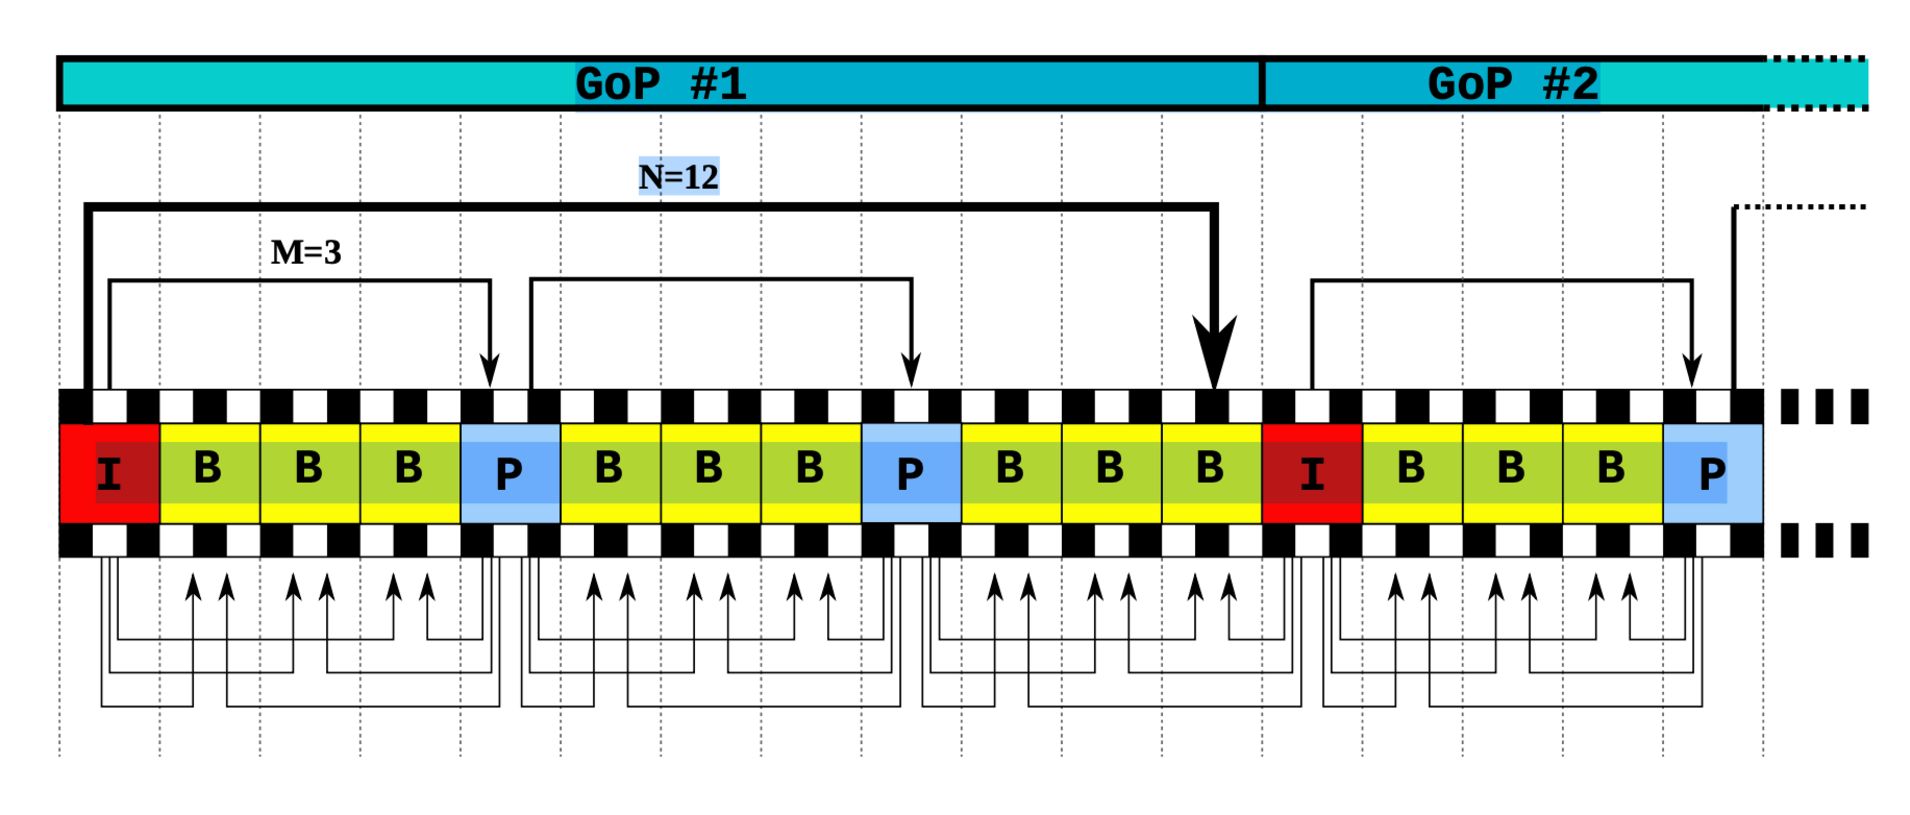
\includegraphics[width=12cm]{Figuras/Figura17}
\end{figure}

La secuencia de fotogramas I, P y B concreta de un vídeo se denomina GoP (group of pictures). En el estándar MPEG-2 suele ser un patrón fijo a lo largo del vídeo, y el más común es el N=12/M=3, donde N es la longitud del GoP, y M es el número de imágenes B entre dos imágenes I o P, como en la figura. El estándar MPEG-4 no suele llevar un patrón fijo para el GoP, sino que el propio codificador determina el tipo de fotograma de forma dinámica.



\section{Propiedades de las imágenes}

Para trabajar con imágenes digitales, emplearemos el programa GIMP. Para empezar, abra con GIMP una imagen cualquiera, y obtenga sus propiedades fundamentales, mediante:
\begin{itemize}
\item Imagen $\rightarrow$ Propiedades de la imagen...
\end{itemize}

Comprobar y anotar en la memoria las siguientes propiedades:
\begin{itemize}
	\item Dimensiones (alto y ancho en píxeles).
	\item Espacio de color (RGB; escala de grises, ...).
	\item Resolución (en ppp).
	\item Tamaño de impresión (Dimensiones / resolución)
\end{itemize}

Comprobar posteriormente el efecto de la resolución en una imagen cuando se pega sobre un documento. Para ello, guardar la misma imagen con resoluciones 100 ppp (imagen100.jpg) y 200 ppp (imagen200.jpg), mediante:
\begin{itemize}
	\item Imagen $\rightarrow$ Tamaño de la impresión...
	\item Archivo $\rightarrow$ Exportar como...
\end{itemize}


Sobre el documento de la memoria de la práctica pegar ambas imágenes, una debajo de la otra, sin modificar el tamaño de éstas:
\begin{itemize}
	\item Insertar $\rightarrow$ Imagen $\rightarrow$ A partir de archivo...
\end{itemize}

Tenga cuidado de que el tamaño original de la imagen no sea excesivamente grande, para evitar que el propio editor de textos modifique la resolución de ésta para que entre dentro de la página. Si este fuera el caso, puede reducir en primer lugar las dimensiones de la imagen con la instrucción
\begin{itemize}
	\item Imagen $\rightarrow$ Escalar la imagen...
\end{itemize}

y ajustar sus dimensiones a un valor más pequeño. Por ejemplo, cuando ajustemos la resolución a 100 ppp, o lo que es equivalente, 100/2,54=39,37 píxeles por centímetro, teniendo en cuenta que el ancho de impresión de un folio A4 es de unos 20 cm, la imagen no podrá tener un ancho mayor de:

$w<20\cdot 39,37=787 \, pixels$

Compruebe que, aunque ambas imágenes tengan las mismas dimensiones, el tamaño de impresión es distinto, dado que hemos cambiado su resolución.



\section{Paleta de colores del modelo HSV}

En este apartado, vamos a emplear el modelo de color HSV para crear la
imagen de la siguiente figura

\begin{figure}[h!]
  \centering
  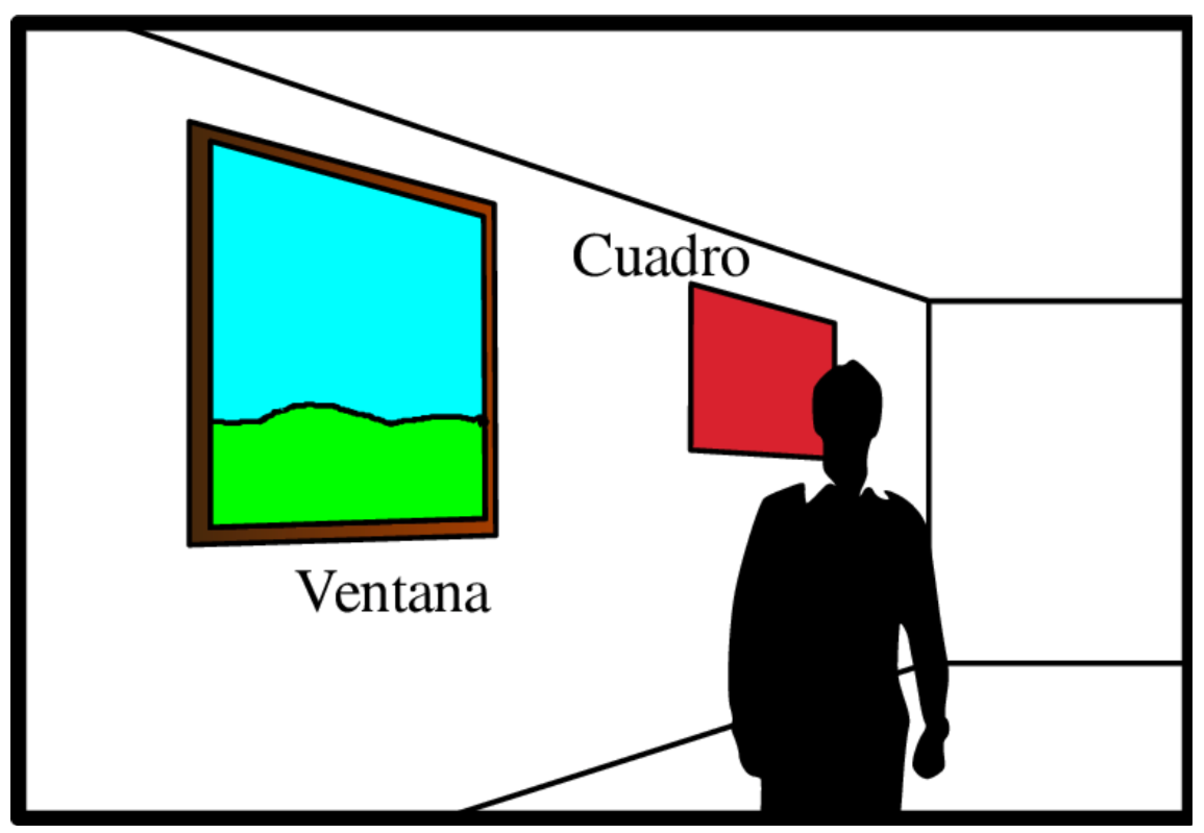
\includegraphics[width=5cm]{Figuras/Figura1}
\end{figure}

Asimismo, veremos alguna herramienta de GIMP que emplearemos en posteriores prácticas. Recordemos que el modelo HSV tiene tres canales. El canal ``valor'' corresponde a la cantidad de luz de cada píxel de la imagen. Este canal sería el equivalente a una imagen en escala de grises, o ``blanco y negro''. El canal ``tono'' se corresponde con el color del píxel. En concreto, para el modelo HSV, un píxel de valor 0 se corresponde con el color rojo. A medida que dicho valor aumenta, el color va pasando por el amarillo, el verde, el cían, el azul, el magenta y vuelta al rojo. Finalmente, el canal ``saturación'' se refiere a la pureza del color, o la cantidad de mezcla con el blanco. En concreto, un píxel con valor 0 sería blanco (o gris en general), y conforme este valor aumenta, el color se vuelve más intenso.

Para crear la figura anterior, vamos a generar un degradado en horizontal para el tono, y un degradado en vertical para la saturación. De esta forma, en la imagen generada, el tono variará en sentido horizontal, mientras que la saturación en vertical. Para ello, seguiremos el siguiente procedimiento:

\begin{enumerate}
	\item Crear una imagen nueva (Archivo $\rightarrow$ Nuevo...), de tamaño 256x256 píxeles.
	\item Descomponer la imagen al espacio de color HSV:
	\begin{itemize}
		\item Colores $\rightarrow$ Componentes $\rightarrow$ Descomponer...
		\begin{itemize}
			\item Modelo de color: HSV
			\item Descomponer en capas: Sí
		\end{itemize}
	\end{itemize}
	\item Para conseguir la variación del color en sentido horizontal, generar un degradado horizontal, sobre la imagen del canal de tono, empleando la herramienta de degradado:
	\begin{itemize}
		\item Herramientas $\rightarrow$ Herramientas de pintura $\rightarrow$ Degradado
	\end{itemize}
	\item Arrastrar con el ratón en sentido horizontal. Para forzar a que el arrastre sea completamente horizontal, pulsar Ctrl mientras se arrastra. Asegurarse de que el color de fondo es blanco, y el de frente negro (Herramientas $\rightarrow$ Colores predefinidos).
	\item Igualmente, para conseguir la variación de la saturación en sentido vertical, generar un degradado vertical sobre la imagen del canal de saturación, empleando la misma herramienta.
	\item Para la imagen del canal de valor, dejarla completamente blanca.
	\item Recomponer la imagen mediante:
	\begin{itemize}
		\item Colores $\rightarrow$ Componentes $\rightarrow$ Recomponer
	\end{itemize}
\end{enumerate}

Posteriormente, modificar la imagen del canal de valor, para dejarla gris. Para ello, pulse sobre el selector del color de frente (rectángulo negro de la figura), y ajústelo a un color gris. Para cambiar el color del canal de valor, seleccione:
\begin{itemize}
	\item Herramientas $\rightarrow$ Herramientas de pintura $\rightarrow$ Relleno
	\item Rellenar la selección completamente
\end{itemize}

Y pulse sobre cualquier punto de la imagen. Recomponer la nueva imagen. En la memoria incluya las imágenes de tono y saturación, las dos imágenes de valor y sus correspondientes imágenes generadas.

\section{Conversión entre espacios de colores}

En este apartado, vamos a emplear el espacio de color HSV para modificar la saturación de una imagen en color. Aunque existe un comando que permite realizar este proceso de forma inmediata (comando Tono y saturación del menú Colores), en este caso vamos a seguir un procedimiento alternativo. Para ello, después de abrir la imagen en color, ejecutamos:
\begin{itemize}
	\item Colores $\rightarrow$ Componentes $\rightarrow$ Descomponer...
	\begin{itemize}
		\item Modelo de color: HSV
		\item Descomponer en capas: Sí
	\end{itemize}
\end{itemize}

Tras la descomposición, obtenemos tres capas, una por cada componente del modelo de color. Para reducir la saturación de la imagen original, únicamente será necesario reducir el valor de los píxeles de la imagen correspondiente al canal de saturación. Recuerde que aunque la imagen original está compuesta por 3 canales (R, G y B), tras la descomposición, cada una de las nuevas imágenes estaría compuesta por un único canal (escala de grises). Para modificar el valor de los píxeles de una imagen, existen distintos procedimientos. Uno de los más sencillos puede ser empleando el comando:
\begin{itemize}
	\item Colores $\rightarrow$ Brillo y contraste...
\end{itemize}

Ajustando el parámetro brillo podemos reducir (o aumentar) el valor de los píxeles en cuestión. Seleccione la imagen correspondiente a la saturación, reduzca su valor, y vuelva a recomponer la imagen, comprobando como la saturación de ésta se ha reducido (ha perdido color, tendiendo a una imagen en blanco y negro). Incluir en la memoria la nueva imagen con la saturación reducida y las tres imágenes correspondientes a los canales del espacio HSV.


\section{Bandas de color y tramado}

La paleta de colores es una técnica empleada para reducir el número de bits por píxel, y por tanto, el tamaño del archivo, a costa de reducir el número máximo de colores disponibles en una imagen. Por ejemplo, para una imagen RGB con 8 bits por canal, el número disponible de colores es igual a $2^{3\cdot 8}=16$ millones de colores (true color). Esto no tiene por qué coincidir con la capacidad de un monitor de reproducir todos esos colores. En general, los monitores reproducen un número menor de colores, y cuanto mejor es la calidad de éste, mayor será la cantidad de colores que pueda reproducir.
Las paletas de colores típicas empleadas por los sistemas audiovisuales reducen el número de bits por píxel a 8, con lo cual tendremos un total de $2^8=256$ colores. De esta forma, hemos reducido el espacio ocupado por la imagen a la tercera parte, con el inconveniente de que, al reducir el número máximo de colores, la calidad de la imagen puede degradarse considerablemente.
La principal consecuencia de la degradación de la calidad de la imagen es la aparición de lo que se denomina como bandas de color. En la siguiente figura se muestra un ejemplo (en este caso, en escala de grises, aunque para imágenes en color el resultado es el mismo). La imagen original (izquierda), con 8 bpp, (256 niveles de grises), se ha reducido a 3 bpp (8 niveles), donde se aprecian claramente las bandas de color (centro).

\begin{figure}[h!]
\centering
\begin{subfigure}
  \centering
  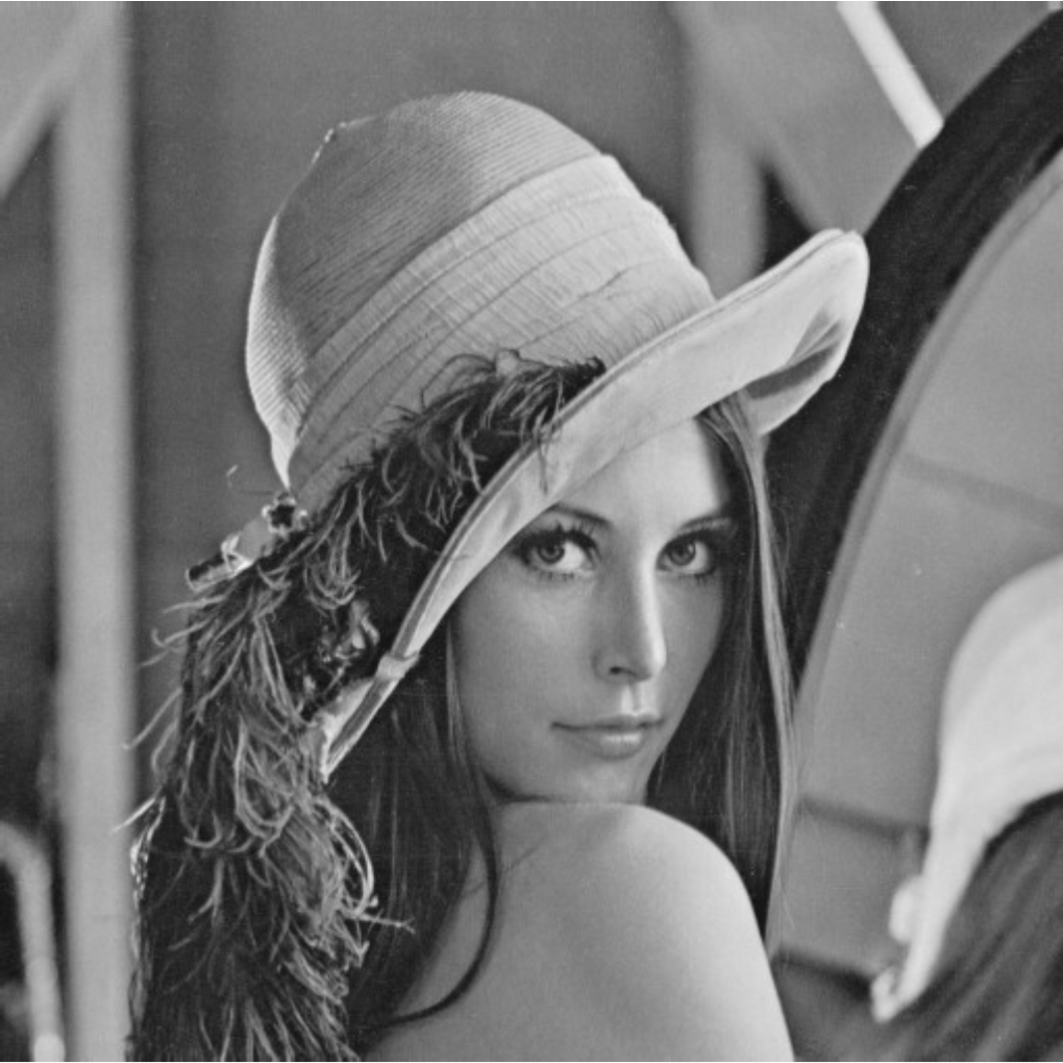
\includegraphics[width=3cm]{Figuras/Figura2}
\end{subfigure}
\begin{subfigure}
  \centering
  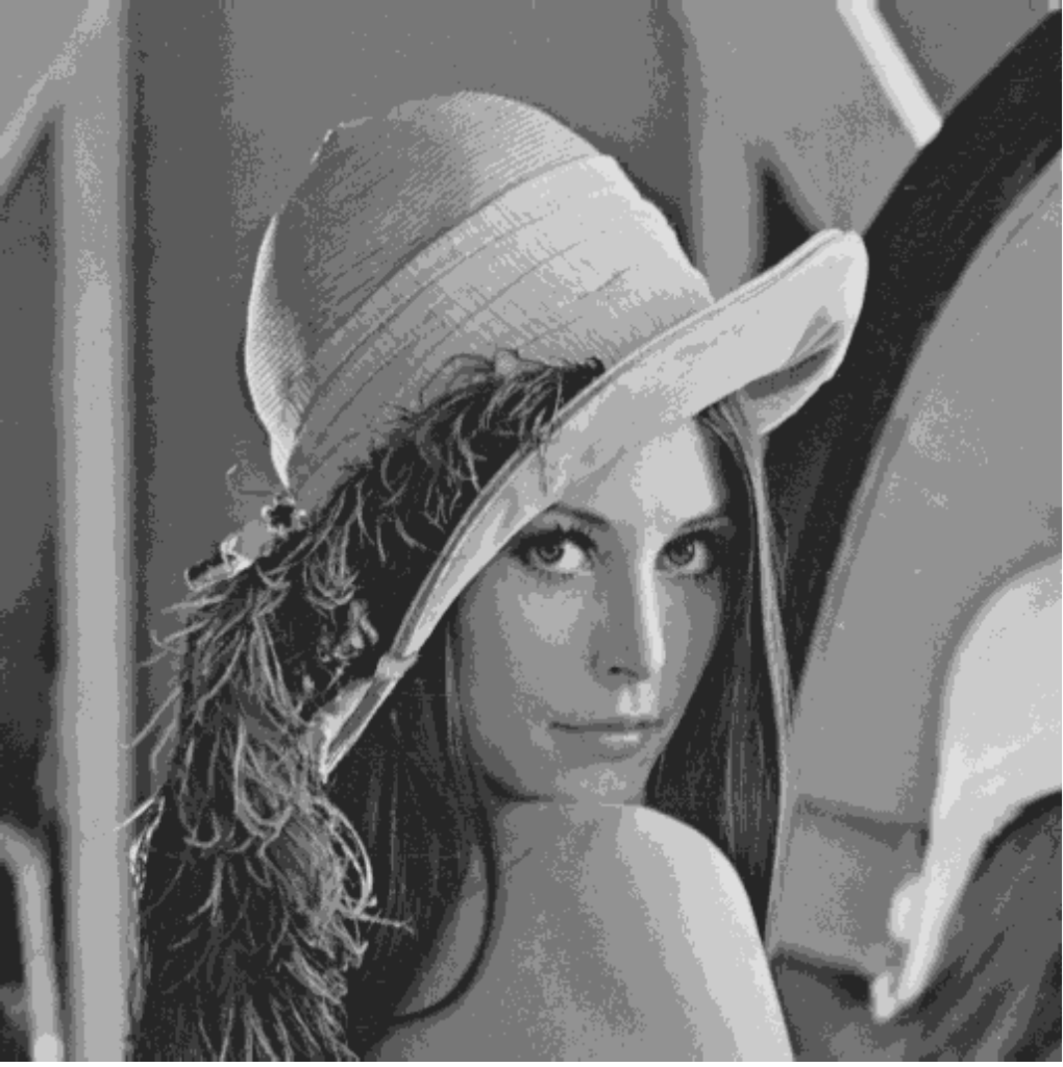
\includegraphics[width=3cm]{Figuras/Figura3}
\end{subfigure}
\begin{subfigure}
  \centering
  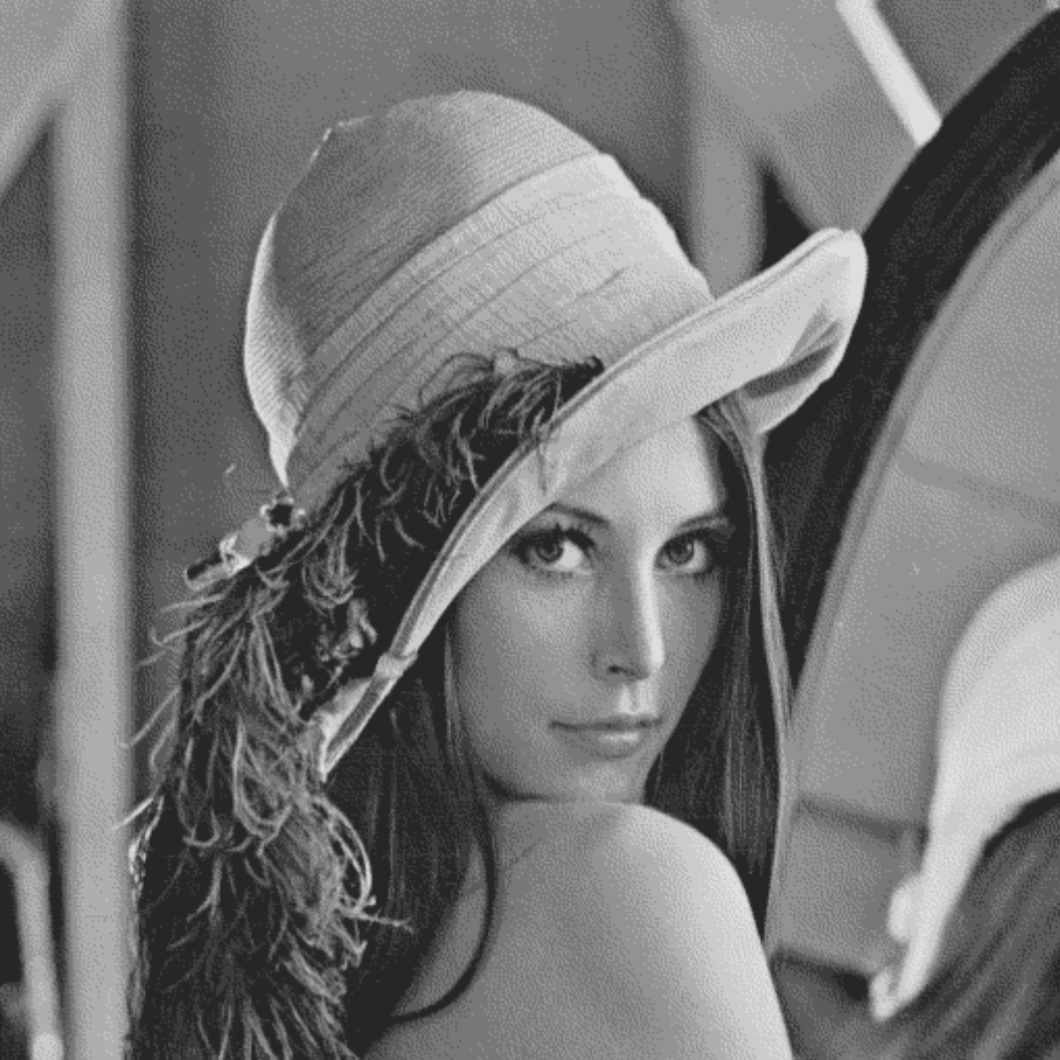
\includegraphics[width=3cm]{Figuras/Figura4}
\end{subfigure}
\end{figure}


El resultado puede mejorarse empleando la técnica denominada como tramado o dithering. Esta técnica trata de simular los colores no disponibles en la paleta de colores mediante la difusión de los colores disponibles en ésta, como puede verse en la figura de la derecha.

Un ejemplo muy típico del uso del tramado son las imágenes en semitonos, o halftones, muy común en impresión mediante tinta (por ejemplo, periódicos). En estos casos, sólo disponemos de dos colores (blanco y negro), de tal forma que si queremos generar un nivel de gris determinado, sólo podemos hacerlo mediante difusión de los dos colores anteriores. En la siguiente figura, se muestra un ejemplo de una figura en semitonos, y un detalle de ésta, donde se puede comprobar cómo realmente la imagen está formada únicamente por dos colores.

\begin{figure}[h!]
	\centering
\begin{subfigure}
  \centering
  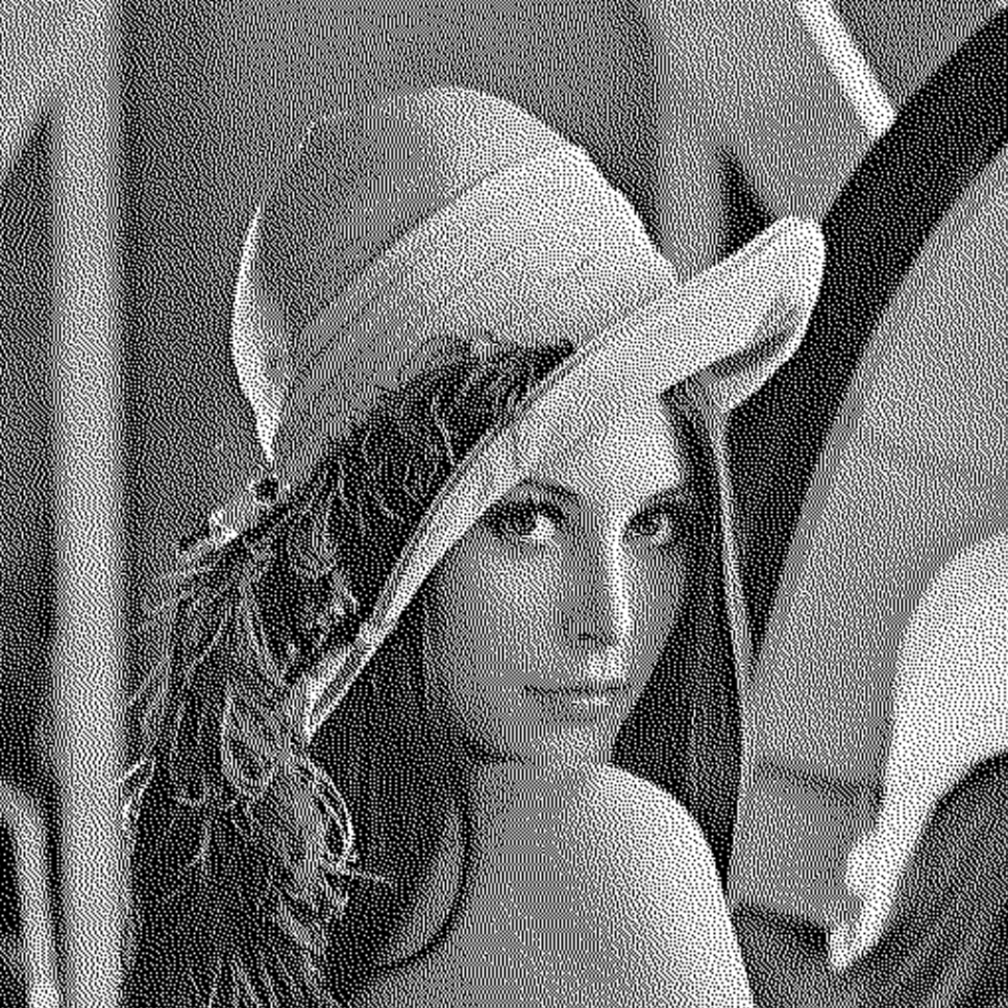
\includegraphics[width=6cm]{Figuras/Figura5}
\end{subfigure}
\begin{subfigure}
  \centering
  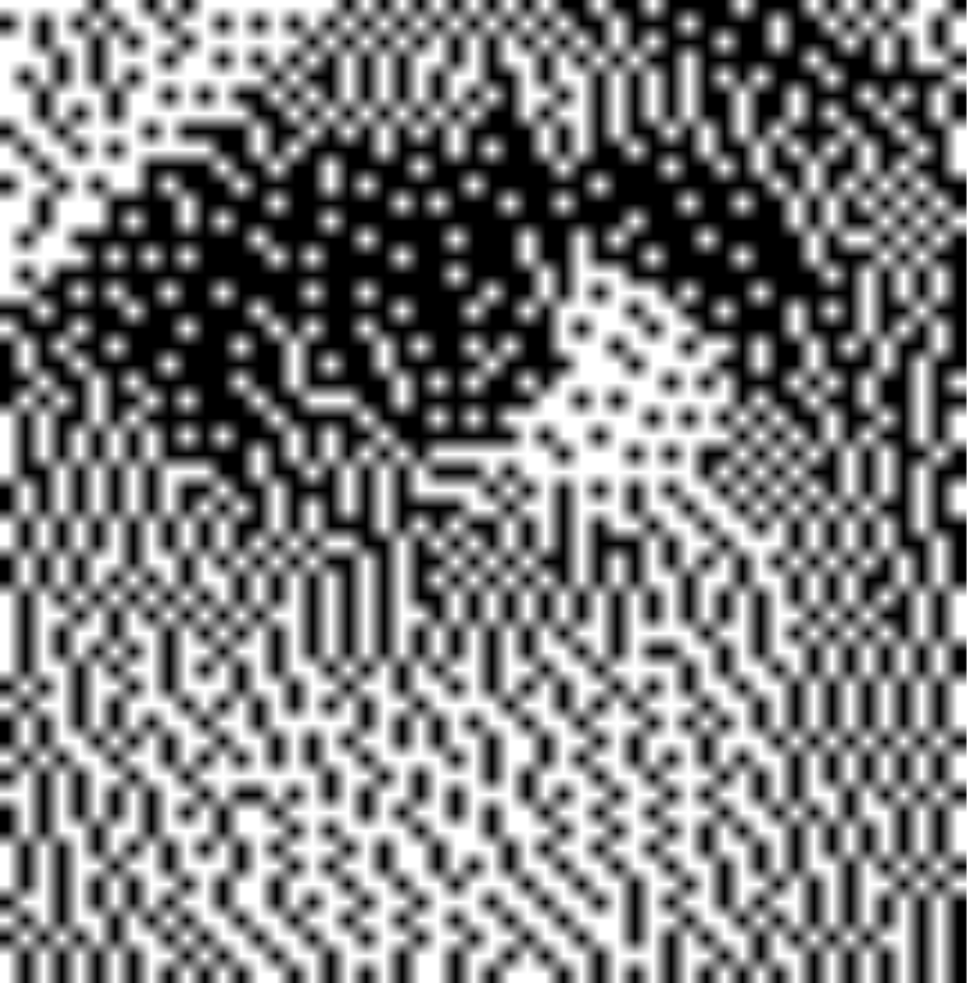
\includegraphics[width=6cm]{Figuras/Figura6}
\end{subfigure}
\end{figure}


Para comprobar el efecto del tramado, abra una imagen en color y reduzca la paleta de colores mediante:
\begin{itemize}
	\item Imagen $\rightarrow$ Modo $\rightarrow$ Indexado
	\item Generar paleta óptima (256 colores)
	\item Tramado (difuminado): ninguno
\end{itemize}

Si el efecto de las bandas de color no se aprecia correctamente, repita el procedimiento, reduciendo el número de colores, de 256 a un valor inferior.

Repita el mismo proceso, pero ahora seleccione, en el campo Tramado, cualquiera de las opciones disponibles. Compruebe el resultado. Incluya en la memoria la imagen original y las dos imágenes generadas.


\section{Formatos de imágenes}

Analizaremos en este apartado los formatos más populares para las imágenes. Para ello, seleccionar una imagen en escala de grises\footnote{Utilice Imagen $\rightarrow$ Modo para comprobar que se trata de una imagen en escala de grises, y si no es así, convertirla.}, y obtener sus parámetros fundamentales (alto, ancho, número de canales y profundidad de bits). Con estos parámetros, calcular el tamaño sin comprimir de la imagen. Posteriormente, guardar la imagen (Archivo $\rightarrow$ Exportar como...) empleando los siguientes formatos:
\begin{itemize}
	\item BMP (sin comprimir)
	\item TIFF (compresión LZW)
	\item PNG
	\item GIF
	\item JPEG (calidad: 90)
	\item JPEG (calidad: 50)
	\item JPEG (calidad: 10)
\end{itemize}

Para cada uno de los formatos anteriores, obtenga la tasa de compresión.

Vamos ahora a emplear un método para poder comparar dos imágenes similares de forma rápida con GIMP. Para ello, abriremos el diálogo de capas:
\begin{itemize}
	\item Ventana $\rightarrow$ Diálogos empotrables $\rightarrow$ Capas
\end{itemize}

Y seguiremos el siguiente procedimiento:
\begin{itemize}
	\item Archivo $\rightarrow$ Abrir... (abrir primera imagen)
	\item Archivo $\rightarrow$ Abrir como capas... (abrir la segunda imagen)
	\item Seleccionar capa superior (en el diálogo de capas)
	\item Modo de la capa: diferencia
	\item Imagen $\rightarrow$ Aplanar la imagen
	\item Colores $\rightarrow$ Info $\rightarrow$ Histograma
\end{itemize}


En el campo Media obtenemos el valor absoluto de la diferencia, mientras que en el campo Desv. Est. el valor cuadrático de la diferencia:
\begin{displaymath}
	m = |i_1 - i_2 |
\end{displaymath}
\begin{displaymath}
	d = \sqrt{(i_1-i_2)^2}
\end{displaymath}

Cualquiera de estos dos valores nos puede servir para obtener una medida de la diferencia entre ambas imágenes. Empleando las imágenes del apartado anterior, compare la imagen original con cada una de las imágenes generadas. Obtenga la relación S/N para cada una de las imágenes. Dicha relación puede obtenerse como:
\begin{displaymath}
	S/N = 20 \cdot log(m)
\end{displaymath}

si empleamos el valor absoluto, o:

\begin{displaymath}
	S/N = 10 \cdot log(d)
\end{displaymath}

si empleamos el valor cuadrático.

Genere una tabla indicando, para cada formato, la tasa de compresión y la relación S/N. Recuerde que si m o d son cero, la relación S/N es infinita.

\begin{center}

\begin{tabular}{|l|l|l|}
\hline
{\bf Formato} & {\bf Tasa de compresión} & {\bf Relación S/N(dB)} \\
\hline	
BMP (sin compresión) & & \\
\hline	
TIFF (compresión LZW) & & \\
\hline	
PNG & & \\
\hline	
GIF & & \\
\hline	
JPEG (calidad 90) & & \\
\hline	
JPEG (calidad 50) & & \\
\hline	
JPEG (calidad 10) & & \\
\hline	
\end{tabular}
\end{center}

Determine qué formatos son sin compresión, que formatos son sin pérdidas, y que formatos son con pérdidas. Incluya en la memoria la imagen original, la tabla anterior, y la respuesta a esta última pregunta.

\end{document}

	
